\chapter{Approach}\label{approach}

\section{Quadrotor Platform}
Because the design and construction of a quadrotor is beyond the scope of  this project, we will use a commercially available vehicle called the Bitcraze Crazyflie \cite{bitcraze}. The Crazyflie, shown in Figure \ref{fig:quad} is a small, low cost, open-source quadrotor kit suitable for indoor flight. It measures 9 cm motor to motor and weighs 19 grams. A 170 mAh lithium-polymer battery powers the vehicle, providing 7 minutes of flight time. An onboard microcontroller is responsible for vehicle stabilization and control and reads sensor measurements from a three-axis accelerometer and a three-axis gyroscope.
\begin{figure}[!htb]
\centering 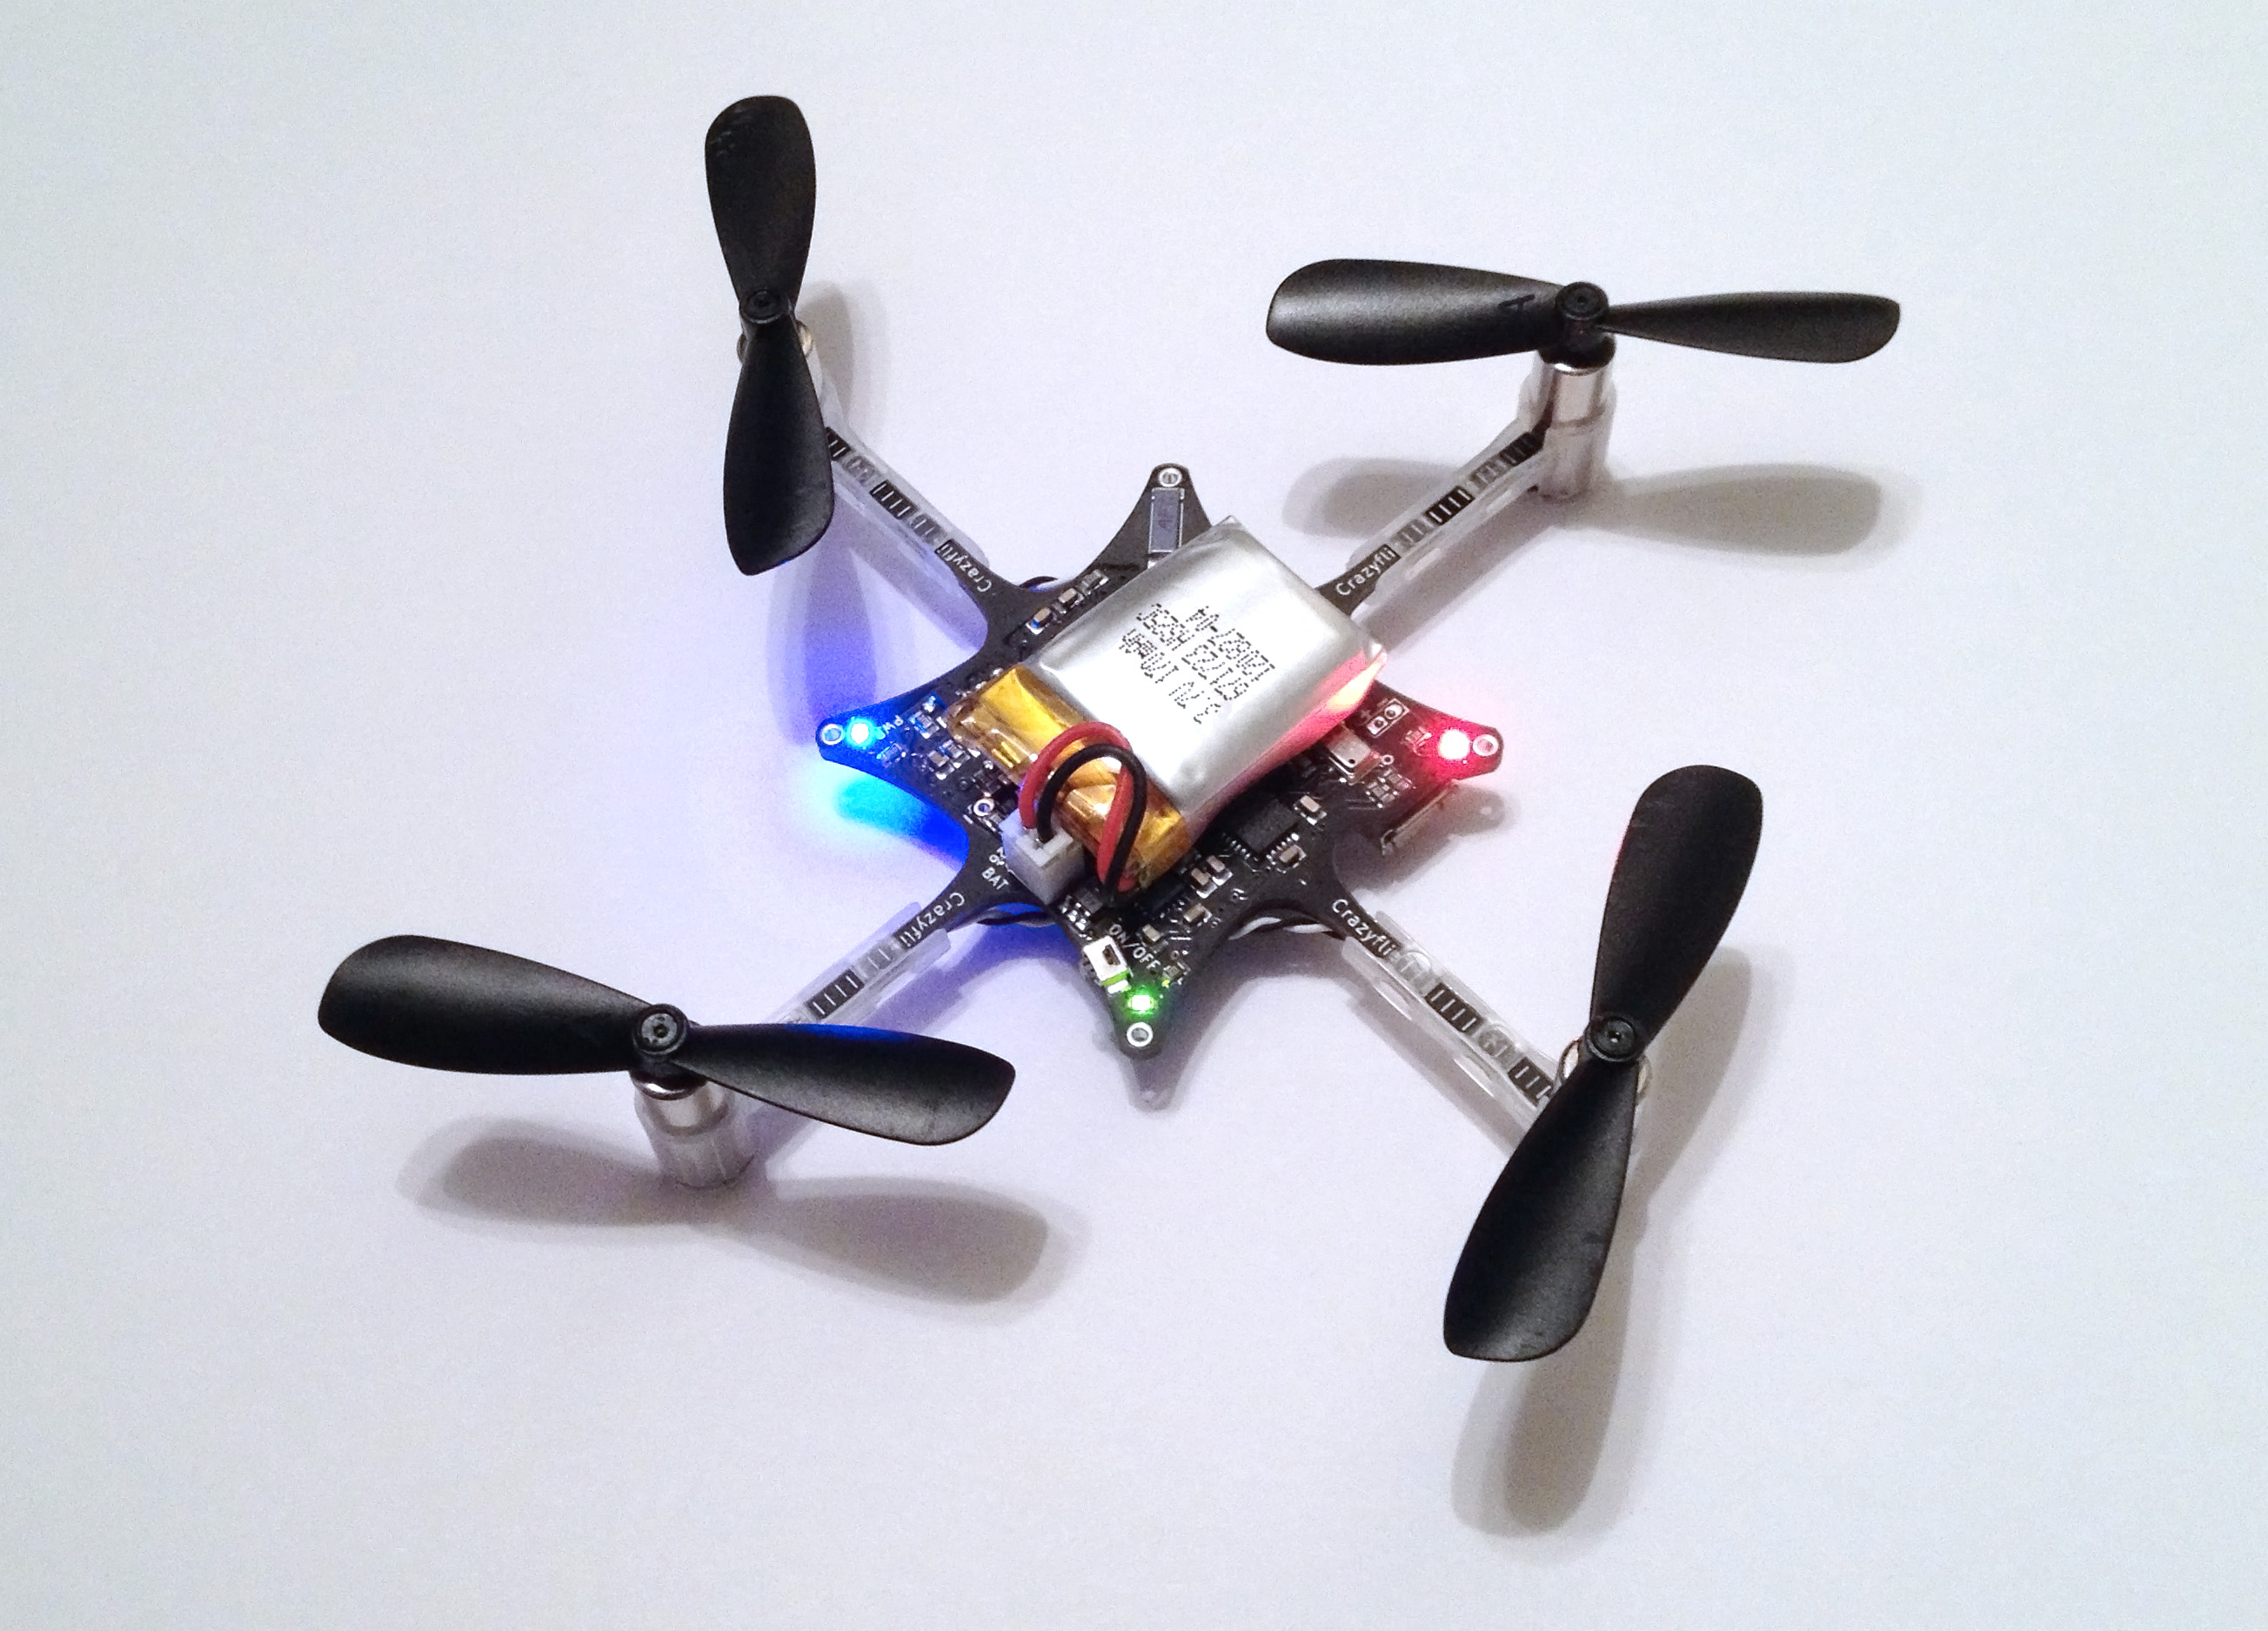
\includegraphics[scale=.11]{../fig/crazyflie.jpg}
\caption{Bitcraze Crazyflie Quadrotor}
\label{fig:quad}
\end{figure}

Vehicle pitch, roll, yaw, and thrust inputs are set in one of two ways. First, a USB gamepad connected to a computer running the Crazyflie PC client provides a method for direct user control of the vehicle. Second, the PC client exposes a Python API, making it possible to programmatically send the vehicle control set-points. The vehicle receives control inputs and transmits telemetry data wirelessly over a 2.4 GHz radio connection to a USB radio dongle connected to the Crazyflie PC client running on a laptop computer.

The onboard stabilization and control system implements an outer-loop attitude controller and an inner-loop rate controller, as shown in Figure \ref{fig:control_system_block_diagram}. Reference pitch and roll commands ($\phi$ and $\theta$, respectively) are fed to the attitude controller (outputting desired rates) and reference yaw rate ($\dot\psi$) is fed directly to the rate controller. The inner-loop rate control operates at 500 Hz and the outer-loop attitude control operates at 250 Hz.
\begin{figure}[htb!]
	\centering
	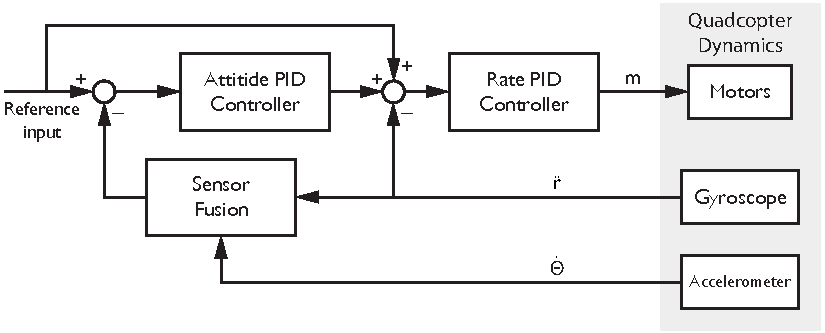
\includegraphics{../fig/crazyflie_control_system_block_diagram.pdf}
	\caption[Crazyflie stabilization and control system block diagram.]{Crazyflie stabilization and control system block diagram where $m = \begin{bmatrix}m_1 & m_2 & m_3 & m_4\end{bmatrix}^T$ is a vector of motor commands, $\ddot{r} = \begin{bmatrix}\ddot{x}&\ddot{y}&\ddot{z}\end{bmatrix}^T$ is a vector of vehicle accelerations, and $\dot\Theta = \begin{bmatrix}\dot{p}&\dot{q}&\dot{r}\end{bmatrix}^T$ is a vector of vehicle angular velocities.}
	\label{fig:control_system_block_diagram}
\end{figure}


\section{Experiment Design}
A crucial step in system identification is experiment design. In order to develop a robust system model, the input sequence must sufficiently excite all system modes to be identified and the sensor data must be sampled fast enough to avoid aliasing. Because the choices made during experiment design have a direct impact on the identified model, it may be necessary to update aspects of the design if the model is found to be insufficient. In this sense, the development of a system model through system identification may be viewed as an iterative process.

\subsection{Input Design}
The input sequence used to excite the system to be modeled plays an important role in solving the identification problem. Common input sequences used for system identification include impulse signals, doublets, white noise sequences, frequency sweeps, and pseudo-random binary sequences \cite{verhaegen2007filtering}. We considered three major factors when selecting an input sequence:
\begin{enumerate}
\item The sequence must be capable of sufficiently exciting all system modes to be identified.
\item The sequence must set the persistence of excitation criteria established in Assumption 4 in Section \ref{sec:closed-loop_subspace_identification}.
\item The sequence must be either simple enough to manually execute or formatted in such a way that it is easily transmitted to the vehicle for execution.  
\end{enumerate}
Considering the above factors, we chose to use the pseudo-random binary sequence (PRBS) as system input. A PRBS signal, shown in Figure \ref{fig:general_prbs}, is persistently exciting to the order of the period of the signal \cite{wilson2005understanding} and is easily transmitted to the Crazyflie quadcopter by sending input sequences through the Python API.
\begin{figure}[htb!]
	\centering
	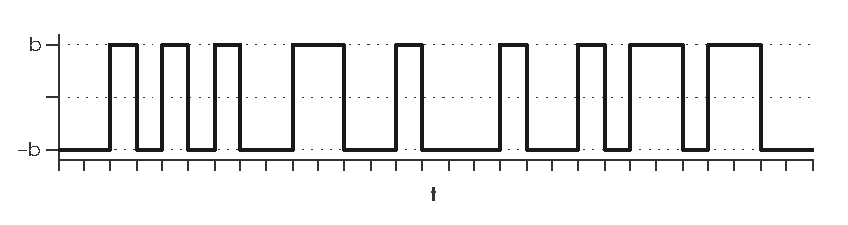
\includegraphics{../fig/general_prbs.eps}
	\caption{A general Pseudo-Random Binary Sequence (PRBS).}
	\label{fig:general_prbs}
\end{figure}

We generated the PRBS signals used for identification by using the \matlab System Identification Toolbox, specifying the signal period to ensure the persistence of excitation criteria is met. Signals were generated for pitch, roll, and yaw rate. Additional input conditioning was performed to appropriately scale the magnitude of the input signal. Scaling factors were experimentally determined to sufficiently excite the vehicle without rendering it uncontrollable.

\begin{table}[!htb]
\centering
\caption{PRBS Scaling Factors}\vspace{1em}
\begin{tabular}{lcc}
\toprule
Input & Maximum & Minimum\\
\midrule
Pitch & $+25^\circ$ & $-25^\circ$\\
Roll & $+25^\circ$ & $-25^\circ$\\
Yaw Rate & $+50^\circ/\mbox{sec}$ & $-50^\circ/\mbox{sec}$\\
\bottomrule
\end{tabular}
\end{table}

\begin{figure}[htb!]
	\centering
	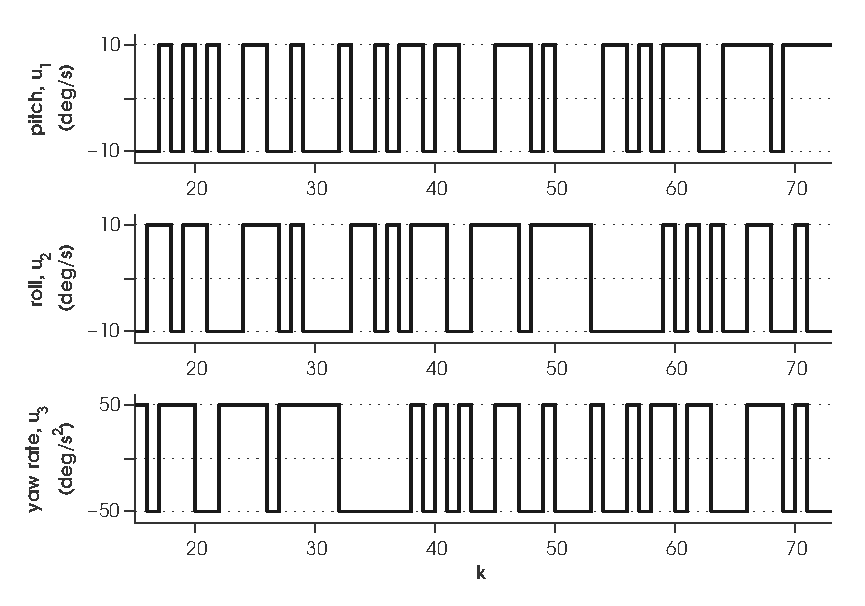
\includegraphics{../fig/test_prbs.eps}
	\caption[A sample PRBS signal used for identification showing scaled inputs for vehicle pitch, roll, and yaw rate.]{A sample PRBS signal used for identification showing scaled inputs for vehicle pitch $= \pm 10^\circ$, roll $= \pm 10^\circ$, and yaw rate $= \pm 50^\circ/\mbox{sec}$.}
\end{figure}

Because the Python API requires system input sequences to be formatted as \{pitch, roll, yaw rate, thrust\}, we also experimentally determined a thrust input which results in vehicle hover. The general flight test sequence is then: vehicle power on and sensor calibration, take off and hover, free flight under PRBS input, landing and vehicle power off. Input signals are sent to the vehicle at 100 Hz. It is worth nothing that the PRBS input does not drive the vehicle directly, instead it acts as a reference input to the controller which in turn commands the vehicle motors. This choice ensures that the vehicle is operating under feedback control and the input-output data gathered is in fact closed-loop data.

\subsection{Data Collection}
System identification requires a rich set of input-output data to identify a suitable model. The Nyquist sampling theorem requires us to sample data at a rate higher than the Nyquist frequency in order to ensure we are able to adequately reconstruct the system input and output signals from logged data. CITE!!!!!!! In the case where the full system dynamics are unknown, it is not trivial to exactly identify the Nyquist frequency. Instead, we sample data at a sufficiently fast rate to identify all system dynamics we are interested in modeling. 

The PC client logging framework provides a means to log system parameters including motor inputs and accelerometer and gyroscope measurements. The Crazyflie PC client communicates with the vehicle and receives logged telemetry data using a custom protocol called the Crazy Real Time Protocol (CRTP). CRTP packets are able to carry a maximum of 31 bytes of data and radio bandwidth is user configurable to either 250 kbps, 1 Mbps, or 2 Mbps. The CRTP protocol is configured to give highest priority to user inputs and as a result, may drop non-essential packets if bandwidth is constrained. In order to maximize data logging ability and minimize dropped log packets, we configure the radio to operate at 2 Mbps. Because the log packets are limited to 31 bytes, we split the logged variables into three separate packets as follows: one log packet contains motor input commands for each of the four motors, one log packet contains $x$, $y$, and $z$ acceleration measurements, and one log packet contains pitch, roll, and yaw rate measurements from the gyroscope. As a result of the packet size limitation and resulting need to transmit logged variables in three separate packets, the fastest we are able to reliably log data is 50 Hz.
\begin{table}[!htb]
\centering
\caption{Logging configuration.}\vspace{1em}
\begin{tabular}{p{7em}p{17em}c}
\toprule
Quantity & Value & Logging Frequency\\
\midrule
Motor inputs & Integers of the input command sent to each of the four motors. Values range from 0 to 64000. & 50 Hz \\[5em]
Accelerometer measurements & Measurements of $x$, $y$, and $z$ accelerations in terms of G's (measured value normalized for gravity) & 50 Hz\\[3em]
Gyroscope \hspace{2em}measurements & Measurements of pitch, roll, and yaw rates in degrees/second. & 50 Hz\\
\bottomrule
\end{tabular}
\end{table}


\section{Data Analysis}
We use the closed-loop input-output data gathered during test flights to construct a system model through the application of a subspace identification algorithm with innovation estimation. Prior to building a model from the sampled data, it is conditioned to provide a more consistent estimate of system dynamics. Following data conditioning, we perform model identification offline using a finite number of sampled data points.


\subsection{Data Preprocessing}
Before identifying a system model, we must first preprocess the data to make it suitable for use. First we trim the beginning and end of the collected input-output sequences to recover only the data collected when the vehicle is driven by PRBS inputs. This process is achieved by simultaneously plotting all input-output data and visually identifying the beginning and end of the data sequences to retain.
\begin{figure}[htb!]
	\centering
	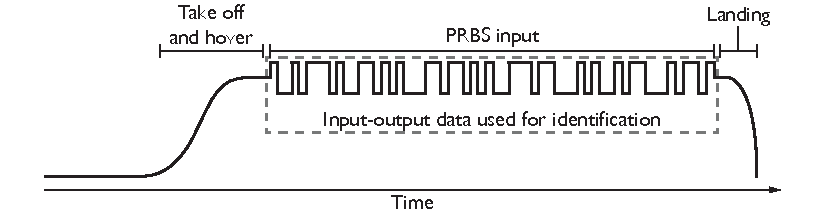
\includegraphics{../fig/test_flight_profile.pdf}
	\caption{Quadrotor test flight profile showing the portion of the test flight data used for system identification.}
	\label{fig:test_flight_profile}
\end{figure}

After extracting the usable segment of the collected data, it must be time normalized. SIMs require the input-output data to be uniformly sampled with data points aligning in time. Because the data we log is captured at slightly different times, we must normalize the sampling times. This is achieved by applying a zero-order hold and resampling the data at a uniform rate of 50 Hz.


\subsection{Model Identification}
We identify a model of the unknown system by applying the general procedure outlined in Table \ref{table:iem_overview}. A \matlab script processes the data offline and presents results when the algorithm is complete. The only user input required is to determine the system order from a plot of the singular values of the extended observability matrix. Selecting only the most significant singular values for inclusion in the model ensures the true system dynamics are captured while reducing the inclusion of noise.

\begin{table}[!htb]\label{table:iem_overview}
\centering
\caption{Overview of the Innovation Estimation Method}\vspace{0.5em}
\fbox{
\begin{minipage}{5.5in}
\begin{enumerate}

\item Recursively estimate the innovation sequence $\hat{E}_i$ row-wise through least squares using
\begin{equation*}
Y_{fi} = \Gamma_{fi}L_p Z_p^T + H_{fi}^- U_{i-1} + G_{fi}^- E_{i-1} + E_{fi}
\end{equation*}

\item Estimate the unknown coefficient matrices row-wise through least squares of
\begin{equation*}
\begin{bmatrix}\hat{\Gamma}_{fi}\hat{L}_p & \hat{H}_{fi}^- & \hat{G}_{fi}^-\end{bmatrix} = Y_{fi}
\begin{bmatrix}Z_p\\ U_{i-1}\\ \hat{E}_{i-1}\end{bmatrix}^\dagger
\end{equation*}
and form the matrix $\hat{\Gamma}_f \hat{L}_p$

\item Estimate the column space of the extended observability matrix from an SVD of $\hat{\Gamma}_f\hat{L}_p$ and appropriately reduce the model order where
\begin{equation*}
\hat{\Gamma}_f = U_1 S_1^{1/2}
\end{equation*}

\item Recover an estimate of $C$ directly from the first block row of $\hat{\Gamma}_f$ and $A$ by solving the least squares problem
\begin{equation*}
\hat{\overline{\Gamma}}_f A = \hat{\underline{\Gamma}}_f
\end{equation*}

\item Recover estimates of $B$ and $D$ by solving the least squares problem
\begin{equation*}
\begin{bmatrix}\mathcal{M}_1\\ \mathcal{M}_2\\ \mathcal{M}_3\\ \vdots\\ \mathcal{M}_f\end{bmatrix} = 
\begin{bmatrix}
\mathcal{L}_1 & \mathcal{L}_2 & \cdots & \mathcal{L}_{f-1} & \mathcal{L}_f\\
\mathcal{L}_2 & \mathcal{L}_3 & \cdots & \mathcal{L}_{f} & 0\\
\mathcal{L}_3 & \mathcal{L}_4 & \cdots & 0 & 0\\
\vdots & \vdots & \ddots & \vdots & \vdots\\
\mathcal{L}_f & 0 & 0 & \cdots & 0
\end{bmatrix}
\begin{bmatrix}I & 0\\ 0 & \hat{\overline{\Gamma}}_f\end{bmatrix}
\begin{bmatrix}D \\ B\end{bmatrix}
\end{equation*}
\end{enumerate}
\end{minipage}}
\end{table}


\section{Model Verification}
Following identification, we verify the system model by simulating system response to an input sequence and comparing its output with data captured from the physical system using the same input sequence. In order to verify the correctness of the identified model and evaluate its overall performance, additional test flights using input sequences not used during identification are conducted. We capture additional input-output data individually exciting the pitch, roll, and yaw dynamics, as well as input-output data showing the coupled dynamics of the system and present a comparison of the real system with the identified model in Chapter \ref{results}.




